\clearpage
\sect{5. El argumento}
Mad Mix ha devuelto la paz a Cocovillage, pero su primo Ope vive una nueva pesadilla en Cococastle. Un coco superviviente se ha refugiado en el castillo y aliado con sus siniestros moradores. Mad debe acudir de nuevo al rescate.


\sect{6. Cómo jugar}
Recorre los pasillos y recoge los cocos para abrirte paso por el castillo. Evita enemigos y trampas; aprovecha el salto para superar obstáculos.

El recorrido tiene nueve fases. Al completar la novena vuelve a la primera. La pantalla anuncia cada fase antes de empezar. Si pierdes una vida, vuelves a la posición inicial de la fase; los cocos ya recogidos siguen recogidos.

Mad permanece centrado mientras el escenario se desplaza a su alrededor; el salto conserva su movimiento vertical.

\textbf{STANDARD} conserva la velocidad habitual. \textbf{HARD} duplica el movimiento base de Mad y los demás actores. El acelerador de Mad tiene el mismo máximo en ambos modos.

\sect{7. La pantalla}
\begin{center}
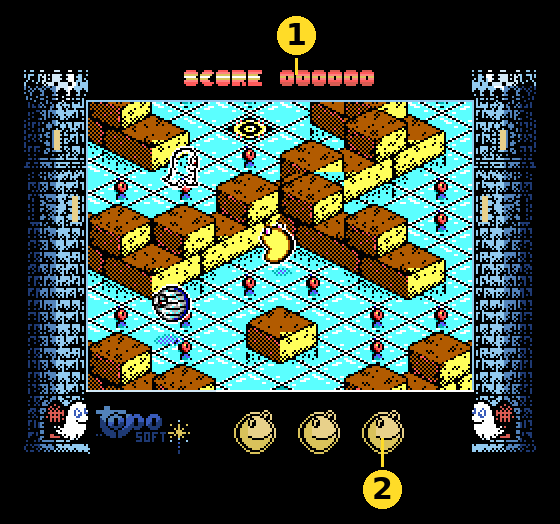
\includegraphics[width=0.68\textwidth]{img/hud.png}
\end{center}
\begin{tabularx}{\textwidth}{@{}clX@{}}
\toprule N.º & Elemento & Qué indica\\\midrule
1 & \texttt{SCORE} & Puntuación acumulada durante la partida.\\
2 & Caras amarillas & Vidas de reserva; la vida que estás usando no se dibuja.\\
\bottomrule
\end{tabularx}

\clearpage
\sect{8. Puntos, vidas y consejos}
Empiezas con una vida activa y tres de reserva. Cuando el marcador queda vacío aún conservas la vida en juego. Las vidas extra pueden aumentar las reservas hasta cuatro.

Un coco normal suma un punto, salvo cuando activa un premio de recogida. Otras recogidas y efectos pueden dar puntuaciones distintas. El contador \texttt{SCORE} se reinicia al comenzar una partida nueva.

\begin{itemize}
\item Al salir de la ilustración inicial, mantén \key{F1} y pulsa Espacio o fuego para evitar el daño por contacto con fantasmas, Drácula y Franky. Las bolas y trampas siguen siendo peligrosas.
\item Pulsa y suelta fuego para cada salto; mantenerlo pulsado no encadena saltos.
\item Empuja los corchos hasta las salidas de los enemigos para bloquearlas temporalmente. Vuelve a alcanzar al acelerador que huye para obtener su impulso.
\item Empuja las bolas contra los monstruos y apártate de su trayectoria cuando rueden.
\item Si necesitas descansar, usa \key{H}. Puedes silenciar la música con \key{V}.
\end{itemize}
